\begin{figure}
	\centering
	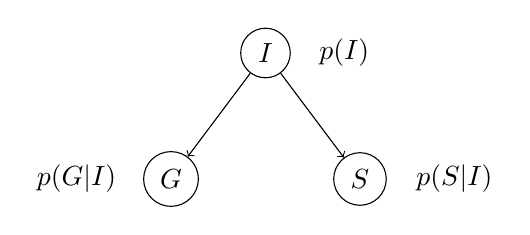
\begin{tikzpicture}[
		scale=0.8
	]

		\node[circle,draw=black] (I) at (0,1) {$I$}; \node at (1.25,1) {$p(I)$};
		\node[circle,draw=black] (G) at (-1.5,-1) {$G$}; \node at (-3,-1) {$p(G \vert I)$};
		\node[circle,draw=black] (S) at (1.5,-1) {$S$}; \node at (3,-1) {$p(S \vert I)$};
		\draw[->] (I) -- (G);
		\draw[->] (I) -- (S);

	\end{tikzpicture}
\end{figure}